%<dscrpt>Complexes et carrés.</dscrpt>
\begin{figure}
 \centering
 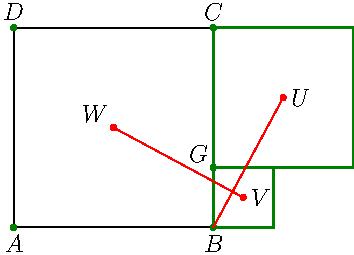
\includegraphics{./Ecomp16_1.pdf}
 % Ecomp16_1.pdf: 0x0 pixel, 300dpi, 0.00x0.00 cm, bb=
 \caption{Construction des carrés extérieurs.}
 \label{fig:Ecomp16_1}
\end{figure}

Soit $ABCD$ un carré et $G$ un point de $\left] B, C \right[ $. On construit deux carrés extérieurs à $ABCD$ de côtés respectifs $\left[ B,G\right]$ et $\left[ G,C\right]$. On note (voir figure \ref{fig:Ecomp16_1})
\begin{itemize}
 \item $U$ le centre du carré de côté $\left[ G,C\right]$,
 \item $V$ le centre du carré de côté $\left[ B,G\right]$,
 \item $W$ le centre du carré $ABCD$. 
\end{itemize}
Le plan est rapporté à un repère orthonormé. On convient que l'affixe d'un point désigné par une lettre majuscule est désignée par la minuscule correspondante.\newline
Ainsi, l'affixe de $A$ est $a=0$, celle de $B$ est $b=1$, celle de $G$ est $g = 1 + \gamma \,i$ avec $\gamma \in \left]  0,1 \right[ $.
\begin{enumerate}
 \item Calculer les affixes $c$, $d$, $u$, $v$, $w$ de $C$, $D$, $U$, $V$, $W$.
 \item Vérifier que les segments $UB$ et $VW$ sont orthogonaux et de même longueur.
\end{enumerate}
